\chapter{راهکار پیشنهادی}\label{chap3}
\minitoc

\section{مقدمه}
در فصول قبل به بررسی روش‌های پیشین پرداخته شد. این روش‌ها شامل رویکرد‌های مختلفی از جمله مدل‌های مبتنی بر \gan{} و یا \vae{} بودند. در ادامه ضمن مروری بر ویژگی‌های کلی مثبت و منفی این دسته از مدل‌ها سعی بر ارائه مدلی است که مزایای هر دو دسته را در بر داشته باشد.
\\
برای شرطی کردن یک مدل زبانی راهکارهای متفاوتی ارائه شد. در ساده‌ترین حالت می‌توان با وارد کردن شرط به یک شبکه \lr{RNN} به یک مدل شرطی دست یافت. این مدل را از دو جهت می‌توان مورد بررسی قرار داد. اول اینکه به دلیل استفاده از روش \teacherforcing{} در آموزش آن، مدل دارای مشکل \expbias{} است. مشکل دوم که شاید نتوان بر روی آن نام مشکل نهاد، مربوط به عدم داشتن فضای نهان است؛ به عبارت دیگر همان طور که در بخش  \ref{chap1:latent_or_not} توضیح داده شد، این دسته از مدل‌ها غیر از مقدار شرط که در ورودی دریافت می‌کنند، ورودی دیگری ندارند و تنها می‌توان با نمونه‌گیری از توزیع نهایی آن‌ها، به نمونه‌های مورد نظر دست یافت. این در حالیست که اگر مدل دارای فضای نهان می‌بود، این امکان وجود داشت تا با حرکت در اطراف یک نقطه از فضای نهان، خروجی مدل را کنترل کرد.
\\
دسته بعدی از مدل‌ها را می‌توان مدل‌های مبتنی بر \gan{} در نظر گرفت. با وجود اینکه مزیت ویژه این دسته از مدل‌ها در داشتن  نمونه‌های با کیفیت است اما از ضعف‌های حائز اهمیتی همچون \modecollapse{} رنج می‌برند \cite{wgan}. این شرایط در حالیست که به دلیل گسسته بودن فضای جملات، در صورت تمایل به استفاده از \gan{}، در انتقال گرادیان نیز مشکل اساسی وجود خواهد داشت که راه حل‌های آن، یا روش‌های تقریبی بوده و یا واریانس آموزشی بالایی دارند. لازم به ذکر است اکثر مدل‌های مبتنی بر \gan{} در حوزه متن نیز بدون فضای نهان هستند. در صورت داشتن فضای نهان نیز از آنجا که امکان رخداد \modecollapse{} وجود دارد، فضای نهان به تعداد محدودی جمله نگاشت شده و عملا نمی‌توان از آن انتظار تفسیرپذیری چندانی داشت.
\\
دسته آخر نیز مربوط به مدل‌های \vae{} است. این مدل‌ها از این جهت که هم دارای فضای نهان با توزیع مشخص هستند و با کران پایینی از معیار \likelihood{} آموزش داده می‌شوند، برخلاف \gan{} دچار مشکل \modecollapse{} نبوده و می‌توان با نمونه‌برداری از فضای نهان (مانند \gan{}) و \decode{} آن‌ها، به جملات رسید. این مدل‌ها نیز بدون ضعف نیستند. همان طور که در بخش \ref{chap1:latent_ignore} و \ref{chap2:latent_ignore} توضیح داده شد، مشکل اساسی \vae{} در تولید متن، عدم توجه به فضای نهان است. راه حل‌های متعددی برای این مشکل ارائه شده است که بعضی آن را ناشی از مشکلات تابع هزینه می‌دانند. علاوه بر این، به دلیل استفاده از روش ‌\teacherforcing{}، این مدل نیز دچار \expbias{} است. گذشته از این ضعف‌ها مشکلات دیگری نیز برای آموزش دادن شرطی این مدل‌ها گزارش شده است؛ مانند این موضوع که مدل به طور همزمان توانایی داشتن خطای بازسازی کم و هم رعایت شرط ورودی را چندان خوب ندارد. احتمالا به همین دلیل است که در \towardctg{} از یک \classifier{} شرط برای اجبار \decoder{} به رعایت شرط استفاده شده است \cite{toward}.

\subsection{مشاهدات رفتار مدل‌های پیشین}
آنچه توضیح داده شد شرح رفتار مدل‌های مختلف بود. در این بخش دو نمونه از رفتارهای نامطلوب دو دسته \gan{} و \vae{} که در آزمایش با آن‌ها مواجه شدیم، توضیح داده خواهند شد.
\\
مدل اول مدل \towardctg{} است که پایه اصلی آن یک مدل \vae{} می‌باشد. نکته حائز اهمیت این دسته از مدل‌ها میزان تاثیر فضای نهان بر خروجی \decoder{} است. در این مدل، از پارامتر $\tau$ (دما) به منظور کنترل میزان اتکای \decoder{} بر فضای نهان استفاده می‌شود. به طور کلی این پارامتر در تغییر دادن یک توزیع گسسته از حالت یکنواخت به ضربه بسیار کاربردی است. اگر $\bff{o}$ بردار ورودی تابع \softmax{} باشد، پارامتر $\tau{}$ که مقداری بین صفر و یک دارد، به صورت زیر تزریق می‌شود:
\begin{gather}
	\bff{y} = \text{softmax}(\bff{o}/\tau) \\
	\bff{x} \sim p_\bff{y} \nonumber
\end{gather}
منظور از $p_\bff{y}$ توزیع گسسته ایست که احتمالات هر مقدار آن مطابق با $\bff{y}$ است. در رابطه فوق اگر پارامتر $\tau$ دارای مقدار یک باشد، تاثیری بر توزیع $\bff{y}$ نداشته و توزیع به حالت قبلی خود باقی می‌ماند؛ اما هر قدر این پارامتر به سمت صفر پیش رود، توزیع خروجی \softmax{} به سمت توزیع ضربه بر روی بیشینه مقدار بردار $\bff{o}$ پیش خواهد رفت و به عبارت دیگر، \greedydecoding{} خواهد بود. \\
در اینجا نیز می‌توان با تغییر این پارامتر میزان تاثیر فضای نهان بر خروجی \decoder{} را اندازه‌گیری نمود. به طور پیش‌فرض مقدار این پارامتر عددی در حدود ۸.۰ قرار داده شده است. با نمونه‌گیری از فضای نهان و \decode{} کردن آن توسط \decoder{} با پارامتر ذکر شده در دو حالت ۸.۰ و نزدیک به صفر، جملات در جدول 
\ref{table:vae_temp_samples}
بدست آمده‌اند.
	\begin{table}[h!]
        \centering
		\begin{tabular}{|c|c|}
            \hline
			\multirow{9}{5em}{\centering \bf{نمونه‌های با پارامتر دمای 8.0}}
           &\lr{a dream cast of solid female talent who build a seamless ensemble .}\\
           &\lr{ what it lacks in originality it makes up for in intelligence and b - grade}\\
            &\lr{a vivid cinematic portrait .}\\
            &\lr{an impeccable study in perversity .}\\
            &\lr{a gift to anyone who loves both dance and cinema}\\
            &\lr{my advice is to skip the film and pick up the soundtrack .}\\
            &\lr{"a twisty , moody slice of southern gothic ..."}\\
            &\lr{and neither nor suspenseful nor particularly well - drawn in by the center .}\\
            &\lr{it 's basically an overlong episode of tales from the crypt .}\\
            \hline
            \multirow{9}{5em}{\centering \bf{نمونه‌های با پارامتر دمای نزدیک به صفر}}
            &\lr{a film that clearly means to preach exclusively to the converted .}\\
            &\lr{a very average science fiction .}\\
            &\lr{the film 's center will not hold .}\\
            &\lr{ very good film sits the place where a masterpiece of the place .}\\
            &\lr{the movie quickly drags on becoming boring and predictable .}\\
            &\lr{a film that clearly means to preach exclusively to the converted .}\\
            &\lr{a film that clearly means to preach exclusively to the converted .}\\
            &\lr{a film that clearly means to preach exclusively to the converted .}\\
            &\lr{a very average science fiction film .}\\
            \hline
		\end{tabular}
		\caption{خروجی مدل  \towardctg 
            در دو حالت با پارامتر دمای 8.0 و نزدیک به صفر.}
        \label{table:vae_temp_samples}
	\end{table}
واضح است در حالتی که منبع عامل تصادفی تنها از فضای نهان باشد، خروجی مدل یک جمله ثابت خواهد بود. بنابراین این طور می‌توان نتیجه‌گیری نمود که خروجی \decoder{} چندان توسط فضای نهان قابل کنترل نیست و تا حدی مستقل کار می‌کند.
\\
مشابه چنین اتفاقی نیز به لحاظ خروجی مدل در مورد \sentigan{} نیز می‌افتد. در اینجا، به دلیل اینکه فضای نهانی وجود ندارد، بنابراین آزمایش پیش‌تر ذکر شده را نمی‌توان انجام داد. اما مشکل اصلی آموزش \gan{} در کنترل میزان آموزش \generator{} و \discriminator{} و رخداد پدیده \modecollapse{} است. روش معمول این دسته از مدل‌ها به این صورت است که ابتدا یک مرحله، \generator{} با معیار بیشینه \likelihood{} 
\trans{\pretrain{}}{Pretrain}
داده شده و پس از آن با تابع هزینه تخاصمی آموزش داده می‌شود.
 	\begin{table}[h!]
     \centering
     \begin{tabular}{|c|c|}
         \hline
         \multirow{9}{5em}{\centering \bf{ابتدای آموزش تخاصمی}}
         &\lr{a bravura exercise in emptiness .}\\
         &\lr{a movie that is without intent .}\\
         &\lr{a sometimes tedious film .}\\
         &\lr{there 's a reason the studio did n't offer an advance screening .}\\
         &\lr{the movie is a desperate miscalculation .}\\
         &\lr{i liked a lot of the smaller scenes .}\\
         &\lr{a film that is a documentary !}\\
         &\lr{it 's a spectacular performance - ahem , we hope it 's a good bark}\\
         &\lr{visually striking and viscerally repellent .}\\
         \hline
         \multirow{9}{5em}{\centering \bf{پس از رخداد \modecollapse{}}}
         &\lr{a movie that 's about as overbearing and over-the-top as the family it depicts .}\\
         &\lr{a movie that 's about as overbearing and over-the-top as the family it depicts .}\\
         &\lr{a movie that 's about as overbearing and over-the-top as the family it depicts .}\\
         &\lr{a movie that 's about as overbearing and over-the-top as the family it depicts .}\\
         &\lr{a warm , and funny , good-natured treat , slight and and funny , good-natured}\\
         &\lr{a film 's a warm and incendiary movie and good-natured treat of the year 's}\\
         &\lr{a film that clearly means to preach exclusively to the converted .}\\
         &\lr{a film that clearly means to preach exclusively to the converted .}\\
         &\lr{a warm , and funny , good-natured treat , slight and and funny and good-natured}\\
         \hline
     \end{tabular}
     \caption{خروجی مدل \sentigan{}
     در ابتدای آموزش تخاصمی و پس از رخداد \modecollapse{}}
     \label{table:gan_modecollapse_samples}
 \end{table}
 به منظور بررسی موضوع ذکر شده، در حین آموزش دو گام، یکی در ابتدای آموزش تخاصمی و دیگری پس از رخداد \modecollapse{} را انتخاب و از مدل نمونه‌برداری و در جدول 
\ref{table:gan_modecollapse_samples}
گزارش شده است. مجددا شاهد وضعیتی هستیم که تنوع جملات تولیدی توسط مدل بسیار کم شده است. لازم به ذکر است که این موضوع با تغییر میزان آموزش \generator{} و \discriminator{} نیز تغییری نکرد.  از آنجا که به ازای هر شرط یک \generator{} جدا در نظر گرفته است، جملات تولیدی هر \generator{} به تعدادی جمله محدود شده و دو دستگی جملات ذکر شده در حالت \modecollapse{} به این علت است (دادگان آموزشی دارای دو مقدار شرط است).
\\
بنابراین در مجموع هیچ کدام از روش‌های فوق خالی از ضعف نیستند اما از آنجا که هدف در این پروژه تولید جملات به صورت شرطی است، به دو شکل می‌توان مدل گرافی برای فضای نهان در نظر گرفت:
\begin{itemize}
    \item
    فضای نهان $\bff{Z}$ تماما توسط مقدار شرط تعیین می‌گردد (شکل \ref{fig:chap3:latent_pgm_h}).
    \item
    فضای نهان $\bff{Z}$ و شرط از یکدیگر مستقل هستند (شکل \ref{fig:chap3:latent_pgm_d}).
\end{itemize}
که بسته به ماهیت \task{}‌ها و دادگان مختلف، می‌توان از هر کدام استفاده نمود.
\begin{figure}[h]
    \centering
    \begin{subfigure}{0.1\textheight}
        \centering
        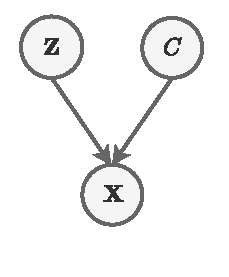
\includegraphics[width=1.\textwidth]{images/pgm_disentangle.pdf}
        \caption{}
        \label{fig:chap3:latent_pgm_d}
    \end{subfigure}
    \hspace{1cm}
    \begin{subfigure}{0.2\textheight}
        \centering
        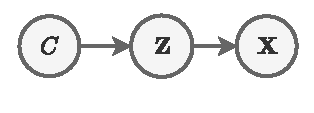
\includegraphics[width=1.\textwidth]{images/pgm_hierarchical.pdf}
        \caption{}
        \label{fig:chap3:latent_pgm_h}
    \end{subfigure}
    \caption{
        دو مدل گرافی متفاوتی که می‌توان برای فضای نهان یک \task{} شرطی در نظر گرفت.
        فضای نهان و شرط مستقل از هم 
        (\subref{fig:chap3:latent_pgm_d})؛
        شرط به طور کامل فضای نهان را تعیین می‌کند
        (\subref{fig:chap3:latent_pgm_h}).
    }
    \label{fig:chap3:latent_pgm}
\end{figure}

\subsection{آموزش \autoencoder{}} \label{chap3:wae_training}
از آنجا که هر دو حالت ذکر شده، مبتنی بر فضای نهان هستند، در طراحی چنین مدلی باید به سوال زیر پاسخ داد:
\begin{itemize}
    \item
    آیا لازم است تا مدلی از خانواده \vae{}  انتخاب شود؟ توزیع حاکم بر فضای نهان چه مزیتی دارد؟
\end{itemize}
برای پاسخ به سوالات فوق لازم است تا هدف و ویژگی‌های مدل‌ها مرور شود. در واقع هدف از داشتن فضای نهان، قابلیت کنترل بر روی فضای نهان و خروجی مدل بود. یکی از این اعمال حرکت بر روی فضای نهان است. حال اگر توزیع مثلا گاوسی بر روی فضای نهان حاکم نباشد، در \autoencoder{}، نقاط به فواصل دوری از هم نگاشت شده و عملا فضا حفره حفره شده و حرکت بر روی آن خروجی مطلوبی نخواهد داشت \cite{infovae}. علاوه بر این جمع کردن فضای نهان جملات در یک توزیع، به دلیل فشرده بودن توزیع هدف، می‌تواند منجر به نزدیک شدن فضای نهان جملات مشابه به یکدیگر شود؛ این در حالیست که همان طور که توضیح داده شد در   \autoencoder{} نقاط نزدیک به هم نگاشت نخواهند شد.
\\
با توجه به دلایل فوق انتخاب یک \autoencoder{} با حاکمیت یک توزیع از پیش تعیین شده بر فضای نهان مبرم به نظر می‌رسد. همان طور که پیشتر اشاره شد \vae{} مشکل عدم توجه به فضای نهان را دارد. به طور کلی راه‌حل‌های ارائه شده برای این مشکل را این طور  می‌توان جمع‌بندی کرد که با وجود اینکه تابع هزینه مورد استفاده در این شبکه‌ها، کران بالایی از منفی لگاریتم \likelihood{} است، اما به طور کلی می‌توان آن را شامل دو بخش بازسازی و منظم‌ساز در نظر گرفت. همان‌طور که در آموزش یک چندجمله‌ای که از تابع منظم‌ساز جمع مجذور وزن‌های تابع استفاده می‌شود و باید میزان توجه و غلبه تابع منظم‌ساز را کنترل کرد، در این مدل‌ها نیز بایستی غلبه بخش \lr{KL} بر بخش بازسازی را کنترل کرد؛ در نتیجه آموزش شبکه سخت خواهد بود. در مقابل یکی از راه‌حل‌های ارائه شده به نام \wae{} با تغییر کوچک تابع هزینه، بخش \lr{KL} را که بین \priordist{} و \posteriordist{} تعریف شده است را به \lr{KL} بین \priordist{} و توزیع حاشیه‌ای \posterior{} تبدیل می‌کند. در نتیجه‌ی این تغییر اثبات می‌کند که تابع هزینه جدید برابر با فاصله \wasser{} بین توزیع داده اصلی و توزیع یادگرفته شده توسط مدل است. توضیح مفصل‌تر این \autoencoder{} و مزیت شهودی آن نسبت به \vae{} در بخش \ref{chap2:wae} آورده شده است.
از سوی دیگر، مقالاتی دیگر به صورت \huristic{}، راه حل‌هایی از جنس اضافه کردن فواصلی بین \priordist{} و توزیع حاشیه‌ای \posterior{} به تابع هزینه \vae{} را ارائه می‌دهند.  بنابراین پاسخ سوال مثبت بوده و از \wae{} استفاده خواهد شد.


\section{مدل پیشنهادی ۱: شرط به طور کامل فضای نهان را تعیین کند}
در حالتی که فضای نهان به طور کامل توسط مقدار شرط تعیین می‌گردد، اگر بتوان فضای نهانی با قابلیت تفسیرپذیری بالا به وجود آورد، این امکان وجود دارد تا در صورت لزوم با یادگیری هر بخش از فضای نهان به یک شرط خاص دست یافت. به عبارت دیگر با یک بار یادگیری فضای نهان، می‌توان از آن برای یادگیری شروط مختلف بهره برد.
\iffalse
 و از آنجا که معمولا داده برچسب خورده برای هر وظیفه‌ای به تعداد زیاد موجود نیست، بنابراین می‌توان انتظار داشت با توجه به کوچکتر بودن فضای نهان نسبت به فضای ورودی، با داشتن فضای نهان تفسیرپذیر، وظایف مربوط به شروط مختلف را حتی با داده کمتری فرا گرفت.
 \fi
\\
در واقع به صورت غیر مستقیم سعی در یادگیری یک \wae{} شرطی داریم؛ به طوری که \encoder{} و \decoder{} شرطی نبوده اما \priordist{} شرطی باشد. در نتیجه \decoder{} شرطی نبوده و مشکل یادگیری همزمان شرط و محتوا وجود نخواهد داشت. در بهترین حالت باید به دنبال تابع هزینه‌ای بود که \priordist{} شرطی را به توزیع \marginal{} \encoder{} نزدیک کند و بالعکس. به طور کلی دو راه برای این رویکرد وجود خواهد داشت. استفاده از \gan{} و یا \mmd{}. از آنجا که \priordist{} صورت مشخصی ندارد بنابراین استفاده از  \mmd{} چندان معقول نخواهد بود. از سوی دیگر استفاده از \gan{} نیز مشکل \modecollapse{} و سایر مشکلات ذکر شده را در پی دارد. بنابراین راه همواری برای نزدیک کردن دو توزیع به یکدیگر وجود ندارد؛ به طوری که گاهی \priordist{} به توزیع \marginal{} \encoder{} نزدیک شود و گاهی بالعکس. به همین دلیل تنها راه این خواهد بود که پس از اتمام آموزش \autoencoder{} ثابت شده و یک مولد شرطی برای فضای نهان هر مقدار شرط یاد گرفته شود. حال می‌توان برای یادگیری توزیع فضای نهان شرطی از \normalizingflownet{} و تابع هزینه \maxlikelihood{} بهره برد. از آنجا که ممکن است ظرفیت مدل مولد شرطی فضای نهان کمتر از پیچیدگی فضای نهان شروط مختلف باشد، برای کاهش اثر \meanseeking{} تابع هزینه \maxlikelihood{}، سعی می‌شود تا توزیع \marginal{} \encoder{} با توجه به مقادیر شرط جدا‌پذیر بوده و تا حدی اثر پدیده فوق تقلیل پیدا کند.
\\
\begin{figure}[h]
    \centering
    \begin{subfigure}{0.6\textheight}
        \centering
        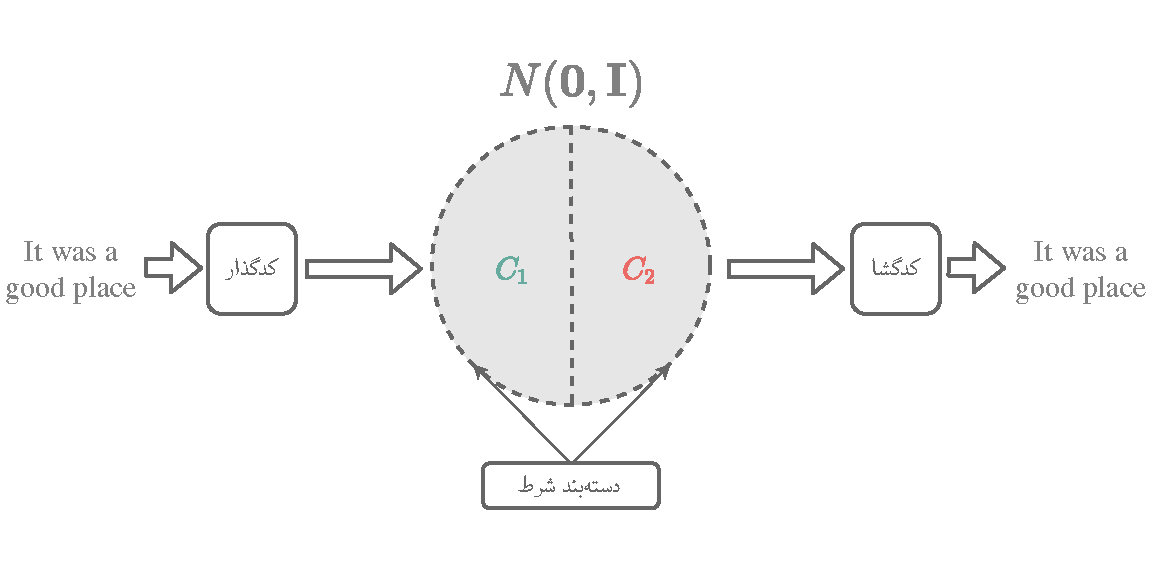
\includegraphics[width=1.\textwidth]{images/propwae.pdf}
        \caption{
            آموزش \autoencoder{} به صورتی که ضمن طبعیت فضای نهان از توزیع گاوسی نرمال، نسبت به مقادیر شرط جدایی پذیر باشد.
        }
        \label{fig:chap4:propwae}
    \end{subfigure}
    \begin{subfigure}{0.5\textheight}
    \centering
    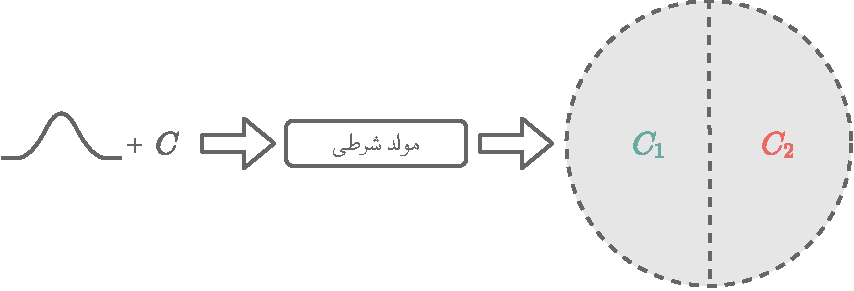
\includegraphics[width=1.\textwidth]{images/propflow.pdf}
    \caption{
پس از مرحله آموزش \autoencoder{} و ساخته شدن فضای نهان مطلوب، یک مدل مولد شرطی فضای نهان آموزش داده خواهد شد. این مدل با دریافت \noise{} و مقدار شرط، برداری در فضای نهان مربوط به مقدار شرط، تولید خواهد نمود.
    }
    \label{fig:chap4:propflow}
\end{subfigure}
\caption{نمایی از مدل پیشنهادی اول}
    \label{fig:chap4:prop}
\end{figure}
بنابراین همان طور که در شکل \ref{fig:chap4:prop} نشان داده شده است، مدل نهایی از دو بخش کلی تشکیل شده است:
\begin{itemize}
	\item \autoencoder{}:
	      این بخش وظیفه ساختن فضای نهان را بر عهده دارد. در این بخش سعی بر این است تا ضمن یادگیری یک مدل مولد جمله، فضای نهان تفسیرپذیر نسبت به شرط نیز یاد گرفته شود. همان‌طور که ییش‌تر توضیح داده شد، \vae{} در یادگیری همزمان بازسازی جمله و رعایت شرط چندان موفق نیست و حذف عامل شرطی از آموزش \decoder{} می‌تواند باعث رفع این دغدغه گردد.
	\item
	      مولد شرطی: این بخش وظیفه یادگیری یک زیرفضا از فضای نهان که مربوط به شروط مورد نظر است را بر عهده دارد.
\end{itemize}
در ادامه به شرح جزئیات این دو بخش پرداخته خواهد شد.

\subsection{آموزش \wae}
به منظور تبیین صوری تابع هدف، اگر $‎q‎$  و $G$ به ترتیب توابع \encoder{} و \decoder{} باشند، خواهیم داشت:
\begin{gather}
	\mathcal{L}_{\text{WAE}}(q, G) = \expected_{\bff{x} \sim p_{\text{Data}}}\expected_{\bff{z} \sim q(\bff{Z}|\bff{x})} [c(\bff{x}, G(\bff{z}))] + \lambda . D_\bff{Z}(q_\bff{Z}, p_\bff{Z})
\end{gather}
که $c(.,.)$ یک تابع فاصله در فضای ورودی و  $D_Z(. , .)$ هم هر فاصله‌ای بین دو توزیع $q_\bff{Z}$ و $p_\bff{Z}$ است. $q_\bff{Z}$ نیز توزیع حاشیه‌ای حاصل از \encoder{} است؛ به عبارت دیگر:
\begin{gather}
	q_\bff{Z}(\bff{Z}) = \sum_\bff{x} p_{\text{Data}}(\bff{x}) q(\bff{Z}|\bff{x})
\end{gather}
در مقاله اصلی، دو گزینه استفاده از \gan{} و فاصله \mmd{} به عنوان $D_\bff{Z}(.,.)$ پیشنهاد شده است که مجددا به دلیل امکان رخداد \modecollapse{} از \mmd{} بهره برده خواهد شد.
اما به جای $c(.,.)$ نیز بایستی از تابع هزینه مناسبی استفاده نمود. بنابر مقاله توضیح داده شده در بخش \ref{chap2:arae}، اگر تابع $p_\psi$ تابعی از فضای نهان $\bff{Z}$ به فضای احتمال جملات با حداکثر طول مشخص
(فضای خروجی $p_\psi$ یک
\trans{\simplex}{Simplex}
$|V|^m-1$
بعدی است که $m$ حداکثر طول جملات و $|V|$ نیز اندازه واژگان است) و
$G(\bff{Z}) = \argmax_{\bff{x}} p_\psi(\bff{x}|\bff{Z})$
، استفاده از تابع هزینه
$\text{cross-entropy}(p_\psi(\bff{X}|\bff{z}), \bff{x})$
به جای $c(.,.)$،
$\mathcal{L}_{\text{WAE}}(q, G)$
کران بالایی برای فاصله \wasser{} بین توزیع داده‌ها و خروجی مدل است. از آنجا که تابع $G$ به صورت \argmaxphrase{} تعریف شده است، از \greedydecoding{} در \decoder{} که تقریبی از \argmaxphrase{} است استفاده می‌شود.
بنابراین تابع هزینه نهایی به شکل زیر است:
\begin{gather}
	\mathcal{L}_{\text{WAE}}(q, p_\phi) = \expected_{\bff{x} \sim p_{\text{Data}}}\expected_{\bff{z} \sim q(\bff{Z}|\bff{x})} [-\log p_\phi(\bff{x}|\bff{z})] + \lambda_\text{MMD} . \text{MMD}(q_\bff{Z}, p_\bff{Z})
\end{gather}
\iffalse
تا به اینجا همچنان مشکل \expbias{} وجود دارد. همان طور که توضیح داده شد، توزیع $Q_Z$ حاصل از حاشیه‌سازی با $P_\text{Data}$ است و به \priordist{} نزدیک می‌شود. حال اگر $Q_Z$ از حاشیه‌سازی  با هر توزیعی غیر از $P_\text{Data}$ بدست آید، دیگر نزدیک به \priordist{} نخواهد بود. با استفاده از این موضوع می‌توان تابع هزینه دیگری نیز برای تقلیل معضل \expbias{} ارائه داد. اگر خروجی \decoder{} به هر دلیلی از توزیع $P_\text{Data}$ فاصله داشته باشد، توزیع $Q_Z$ حاصل از حاشیه‌سازی با ?? نزدیک به \priordist{} نیست و \decoder{} بایستی سعی در تولید جملاتی داشته باشد تا مجموعه آن‌ها در فضای نهان توزیعی نزدیک به \priordist{} را بسازند. این تابع هزینه را به شکل زیر می‌توان صورت‌بندی کرد:
\begin{gather}
	\mathcal{L}_\text{ExpBias}(G) = \lambda_{e} . D_ Z(Q_Z^G, P_Z)
	\\
	Q_Z^G (z) = \int_{z'} P_Z(z') Q(z|G(z'))
\end{gather}
از آنجا که در روابط هزینه فوق از تابع $\argmax$ استفاده شده است، برای انتقال گرادیان از تقریب \lr{Soft-argmax} بهره برده خواهد شد.  \lr{Soft-argmax} به طور کلی پارامتری به نام $\tau$ دارد که نوع \lr{Straight Through} از به صورت زیر تعریف می‌شود:
\begin{gather}
	\bff{y} = \text{softmax}(\bff{o}/\tau)
	\\
	\bff{u} = \bff{y} - \text{stop-gradient}(\bff{y}) + \text{onehot}(\argmax_{o_i} \bff{o})
\end{gather}
که $\bff{o}$ بردار قبل از اعمال \lr{softmax}
،
$\bff{u}$
بردار خروجی و توابع \lr{onehot} و \lr{stop-gradient} به ترتیب تبدیل‌کننده شاخص به بردار
\trans{\onehot{}}{Onehot}
و قطع‌کننده عبور گرادیان هستند. بنابراین همان طور که از تعریف برداشت می‌شود، در فاز
\trans{\forward{}}{Forward}
هیچ تقریبی وجود ندارد اما در فاز
\trans{\backward{}}{Backward}
گرادیان از طریق تقریب \lr{Soft-argmax}
($\bff{y}$)
منتقل می‌شود.
به منظور آموزش \encoder{} در تفاوت قائل شدن بین توزیع فضای جملات واقعی و فضای جملات تولید شده توسط \decoder{} می‌توان تابع هزینه زیر را نیز در نظر گرفت:
\begin{gather}
	\mathcal{L}_\text{ExpBias}(Q) = -\lambda_{e} . D_ Z(Q_Z^G, P_Z)
\end{gather}
\fi
پیش‌تر بررسی شده است که آموزش مدل فوق، در صورتی که خروجی \encoder{} یک توزیع گاوسی باشد، به سمت صفر کردن واریانس این توزیع و عملا قطعی کردن خروجی \encoder{} و حفره حفره شدن فضای نهان خواهد رفت. برای جلوگیری از این موضوع، از فاصله \lr{KL} بین توزیع گاوسی خروجی \encoder{} و توزیع گاوسی با همان میانگین اما واریانس یک استفاده می‌شود \cite{wasser_text_kl}. به عبارت دیگر تابع هزینه زیر افزوده خواهد شد:
\begin{align}
    \mcal{L}_\text{STD} =& \lambda_\text{STD} ~ \expected_{\bff{x} \sim p_\text{Data}} [
    KL(N(\bff{\mu}_{q(\bff{Z}|\bff{x})}, \bff{\sigma}_{q(\bff{Z}|\bff{x})}) ~ || ~ N(\bff{\mu}_{q(\bff{Z}|\bff{x})}, \bff{I}) ) ] \nonumber
    \\
    =& \lambda_\text{STD} ~ \expected_{\bff{x} \sim p_\text{Data}} [ 
    -\log \bff{\sigma}_{q(\bff{Z}|\bff{x})} + \frac{1}{2} \bff{\sigma}_{q(\bff{Z}|\bff{x})}^2 ] + \text{const}
\end{align}
از آنجا که انتظار دسته شدن جملات با توجه به مقدار شرط در فضای نهان، شاید انتظار بالایی باشد، از یک \classifier{} خطی شرط در فضای نهان استفاده خواهد شد تا \encoder{} جملات را به نحوی \encode{} کند تا \classifier{} بتواند آن‌ها را دسته‌بندی کند. بنابراین اگر \classifier{} را با $q_L(c|\bff{z})$ نشان دهیم، تابع هزینه آموزش \classifier{} به شرح زیر است.
\begin{align}
    \mcal{L}_\text{CLS} (q_L) = -\expected_{(\bff{x}, c) \sim p_\text{Data}(\bff{X},C) , \bff{z} \sim q(\bff{Z}|\bff{x})} \log q_L(c | \bff{z})
\end{align}
از سوی دیگر تابع هزینه زیر نیز به تابع هزینه \encoder{} اضافه خواهد شد:
\begin{align}
\mcal{L}_\text{CLS} (q) = - \lambda_\text{CLS} ~ \expected_{(\bff{x}, c) \sim p_\text{Data}(\bff{X},C) , \bff{z} \sim q(\bff{Z}|\bff{x})} \log q_L(c | \bff{z})
\end{align}
که همان تابع هزینه \classifier{} است و \encoder{} را به \encode{} جملات در فضاهای نسبتا مجزایی با توجه به مقدار شرط سوق خواهد داد.

\subsection{آموزش مولد شرطی}
تا به اینجا در مورد نحوه ساختن یک مدل مولد غیر شرطی اما با فضای نهان مناسب صحبت شد. حال با داشتن فضای نهان بایستی مدل مولد شرطی را آموزش داد تا با گرفتن مقدار شرط، توزیعی بر روی فضای نهان دارای شرط مورد نظر بسازد.
\\
از آنجا که فضای نهان، یک فضای پیوسته است، بنابراین بایستی کمی در مورد نحوه انتخاب مدل مولد و روش آموزش آن تامل کرد. همان‌طور که پیشتر توضیح داده شد، موفق‌ترین مدل‌های مولد، \gan{} و \vae{} هستند. در مورد \gan{} که مشکل \modecollapse{} وجود دارد و در مورد \vae{} نیز از آنجا که فضای ورودی آن فضای نهان جملات است، بایستی برای این فضا، فضای نهان دیگری را بسازد. بنابراین این روش‌ها چندان معقول نیستند. در کنار این روش‌ها رویکرد دیگری نیز وجود دارد که چندان به آن توجه نمی‌شود. یادگیری مدل مولد بر پایه بیشینه کردن مستقیم \likelihood{}. از آنجا که در حال صحبت از فضای پیوسته هستیم، بنابراین بایستی از توزیع‌های پارامتری از پیش تعریف شده مانند گاوسی و یا در بهترین حالت از
\trans{\gaussianmix{}}{Gaussian mixture}
استفاده کرد. از آنجا که فرضی بر توزیع فضای نهان یک شرط خاص نداریم، بنابراین به کار بستن چنین مدل‌هایی چندان معقول به نظر نمی‌رسد. همان طور که در بخش \ref{chap2:flow}‌ توضیح داده شد، نوع دیگری از خانواده‌های مولد وجود دارند که هم امکان محاسبه \likelihood{} در خروجی را دارند و هم فرم مشخصی مانند توزیع گاوسی ندارند. به این دسته از شبکه‌ها \normalizingflownets{} می‌گویند. توضیحات مفصلی در رابطه با معرفی این مدل‌ها در بخش \ref{chap2:flow} ارائه شده است و در اینجا صرف نظر می‌شود.
\\
فرض کنید مدل مولد شرطی را با $p_F(\bff{z}|c)$ که یک شبکه از خانواده \normalizingflownets{} است، نشان داده و مجموعه دادگان آموزشی
$\mathcal{X}_C = \{(\bff{x}_i, c_i)\}_{i=1}^{N}$
باشد. اگر
\begin{gather}
	q(\bff{Z}, \bff{X}|c) = p_\text{Data}(\bff{X}|c) q(\bff{Z}|\bff{X})
	\\
	q(\bff{Z}|c) = \sum_\bff{x} q(\bff{Z}, \bff{x}|c)
    = \sum_\bff{x} p_\text{Data}(\bff{x}|c) q(\bff{Z}|\bff{x})
\end{gather}
خواهیم داشت:
\begin{align}
	\mathcal{L}_c (F) = & KL\big(q(\bff{Z}|c) ~ || ~ p_F(\bff{Z}|c)\big) \nonumber                                          \\
	=                   & \int_\bff{z} q(\bff{z}|c) \log \frac{q(\bff{z}|c)}{p_F(\bff{z}|c) \nonumber}                                  \\
	=                   & -\int_\bff{z} q(\bff{z}|c) \log p_F(\bff{z}|c) + \text{const} \nonumber                                 \\
	=                   & -\int_\bff{z} \sum_\bff{x} p_\text{Data}(\bff{x}|c) q(\bff{z}|\bff{x}) \log p_F(\bff{z}|c) + \text{const} \nonumber       \\
	\Rightarrow
	\mathcal{L}_c (F) = & - \expected_{\bff{x} \sim P_\text{Data}(\bff{X}|c), \bff{z} \sim q(\bff{Z}|\bff{x})} [\log p_F(\bff{z}|c)] + \text{const}
\end{align}
رویکرد‌های متفاوتی نیز برای مدل کردن تابع $F$ وجود دارد؛ اما  همان طور که پیشتر توضیح داده شد، مدل‌های \autoregressive{} از این خانواده به مراتب توانایی مدل‌سازی بیشتری دارند و نقطه ضعف آن‌ها در عدم امکان موازی‌سازی بر روی بُعد است؛ اما از آنجا که ابعاد فضای نهان کوچک است، این نکته چندان مشکل‌ساز نیست. دو نوع ساده از این خانواده \lr{MAF} و  \lr{IAF} است. به دلیل آنکه \lr{IAF} و \lr{MAF} توابع معکوس یکدیگر هستند، \lr{MAF} در ادامه توضیح داده خواهد شد.
\\
اگر تابع $F(\bff{Z}_0, c)$ را به صورت
 $F = F_L \circ F_{L-1} \circ ... \circ F_1 (\bff{Z}_0, c)$
 باشد که $F_l$ یک لایه از نوع \lr{MAF} بوده، خروجی لایه $l$ ام را با $\bff{Z}_l \in \bb{R}^D$ نشان داده و $\bff{Z}_0$ نمونه‌ای از توزیع پایه  $p_{\bff{Z}_0}$ با قابلیت محاسبه کارای احتمال یک نمونه و همچنین نمونه‌برداری باشد (در اینجا توزیع گاوسی نرمال)، بُعد $i$امِ لایه $l+1$ام به صورت زیر تعریف می‌شود:
\begin{align}
	\bff{Z}^i_{l+1, c} = & \bff{Z}^i_{l, c} * \Theta^{i}_{l,1}(\bff{Z}^{1:i-1}_{l+1, c}, c) + \Theta^{i}_{l,2}(\bff{Z}^{1:i-1}_{l+1, c}, c)
\end{align}
و تابع معکوس نیز می‌تواند به صورت برداری به شرح زیر نوشته شود:
\begin{align}
	\bff{Z}_{l-1, c} =  & F_{l}^{-1}(\bff{Z}_{l,c},c) \nonumber
	\\
	\bff{ Z}_{l-1, c} = &
	\frac{\bff{ Z}_{l,c} - \Theta_{l,2}(\bff{Z}_{l,c}, c)}
	{\Theta_{l,1}(\bff{Z}_{l, c}, c)}
\end{align}
که $\Theta_{l,1}$ و $\Theta_{l,2}$ نیز توابعی هستند که با شبکه عصبی مدل می‌شوند؛ تنها محدودیت این شبکه‌ها در این است که بُعد $i$ام آن تنها باید تابعی از ابعاد $1$ تا $i-1$ باشد. به این هدف، از معماری \lr{MADE} در $\Theta_{l,1}$ و $\Theta_{l,2}$ استفاده می‌شود.
\\
از آنجا که هر بُعد بر حسب بعدهای قبل از خود است، بنابراین ماتریس ژاکوبین نیز مثلثی بوده و دترمینان آن برابر با حاصل‌ضرب اعضای قطر آن است.
\begin{align}
	\Big[ \frac{\partial F_{l+1}}{\partial \bff{Z}_{l,c}} \Big]_{i,i} = \Theta^{i}_{l,1}(\bff{Z}^{1:i-1}_{l+1,c}, c) \nonumber
	\\
	\text{det}\Big[ \frac{\partial F_{l+1}}{\partial\bff{Z}_{l,c}} \Big] = \prod_{i=1}^D \Theta^{i}_{l,1}(Z^{1:i-1}_{l+1, c}, c)
\end{align}
بنابراین \likelihood{} نقطه $\bff{z}_L$ به طوری که 
$\bff{z}_0 = F^{-1}(\bff{z}_L, c)$
 نیز طبق رابطه \ref{eq:flow_target_dist} به صورت زیر محاسبه می‌شود:
\begin{align}
	\log p_F(\bff{z}_L|c) = & \log p_{\bff{Z}_0}(\bff{z}_0) - \sum_{l=1}^L \log (\text{det}[    \frac{\partial F_{l+1}}{\partial \bff{z}_{l,c}}     ]) \nonumber
	\\
	=               & \log p_{\bff{Z}_0}(\bff{z}_0) - \sum_{l=1}^L \sum_{i=1}^D \log \Theta^{i}_{l,1}(\bff{z}^{1:i-1}_{l+1, c}, c) \nonumber
	\\
	=               & \sum_{i=1}^D -\frac{1}{2} \{\bff{z}^i_0\}^2 - \sum_{l=1}^L \sum_{i=1}^D \log (\Theta^{i}_{l,1}(\bff{z}^{1:i-1}_{l+1,c}, c)) + \text{const} \nonumber
	\\
	=               & -\sum_{i=1}^D \frac{1}{2} \{\bff{z}^i_0\}^2 + \sum_{l=1}^L \log (\Theta^{i}_{l,1}(\bff{z}^{1:i-1}_{l+1,c}, c)) + \text{const}
\end{align}
در نهایت رابطه هزینه آموزش مولد شرطی $\mathcal{L} (F)$ به صورت زیر خواهد بود:
\begin{gather}
    \mathcal{L} (F) = \expected_{c \sim p_\text{Data}(c)} \mathcal{L}_c (F) \nonumber 
    \\
    \mathcal{L} (F) = \expected_{(\bff{x},c) \sim p_\text{Data}(\bff{X},C), \bff{z}_L \sim q(\bff{Z}|\bff{x})} [\sum_{i=1}^D \frac{1}{2} \{\bff{z}^i_0\}^2 + \sum_{l=1}^L \log (\Theta^{i}_{l,1}(\bff{z}^{1:i-1}_{l+1, c}, c))] + \text{const}
\end{gather}
که 
$\bff{z}_{l-1,c} = F^{-1}_{l}(\bff{z}_{l,c},c)$ است.

\section{مدل پیشنهادی ۲: فضای نهان و شرط از یکدیگر مستقل باشند}
در این حالت، از آنجا که هر جمله توسط هر دو بردار مقدار شرط و فضای نهان تعیین می‌شود، بنابراین بر خلاف حالت قبل، با یک \decoder{} شرطی مواجه خواهیم بود؛ به این معنی که علاوه بر خروجی \encoder{}، مقدار شرط را نیز ورودی می‌گیرد. اگر بخواهیم طبق تعریف بخش قبل جلو رویم، توزیع \decoder{} به صورت  $p_\phi(\bff{X}|\bff{Z})$ در خواهد آمد و بخش دیگری تغییر نخواهد کرد.
\\
حال برای آنکه فضای نهان مستقل از مقدار شرط باشد، نیاز به بخش جدیدی در تابع هزینه خواهیم بود. از آنجا که مقدار شرط، همواره بخشی از محتوای جمله است، بنابراین ممکن است مقدار شرط در بردار خروجی \encoder{} و در نتیجه فضای نهان کد شود و مانع استقلال فضای نهان از مقدار شرط گردد. به این منظور با اضافه کردن یک \classifier{}، می‌توان به روش تخاصمی مسئله را حل کرد. اگر درفضای نهان، یک \classifier{} شرط داشته باشیم که با گرفتن برداری از فضای نهان، مقدار شرط آن را تعیین کند، \encoder{} می‌تواند به صورت تخاصمی سعی در به اشتباه انداختن \classifier{} در تشخیص برچسب هر بردار کرده و عملا بردار‌های مربوط به مقادیر مختلف شرط را روی هم انداخته و تشخیص آن را سخت کند. نمایی از این مدل در شکل \ref{fig:chap4:prop2} آمده است.
\begin{figure}[h]
    \centering
        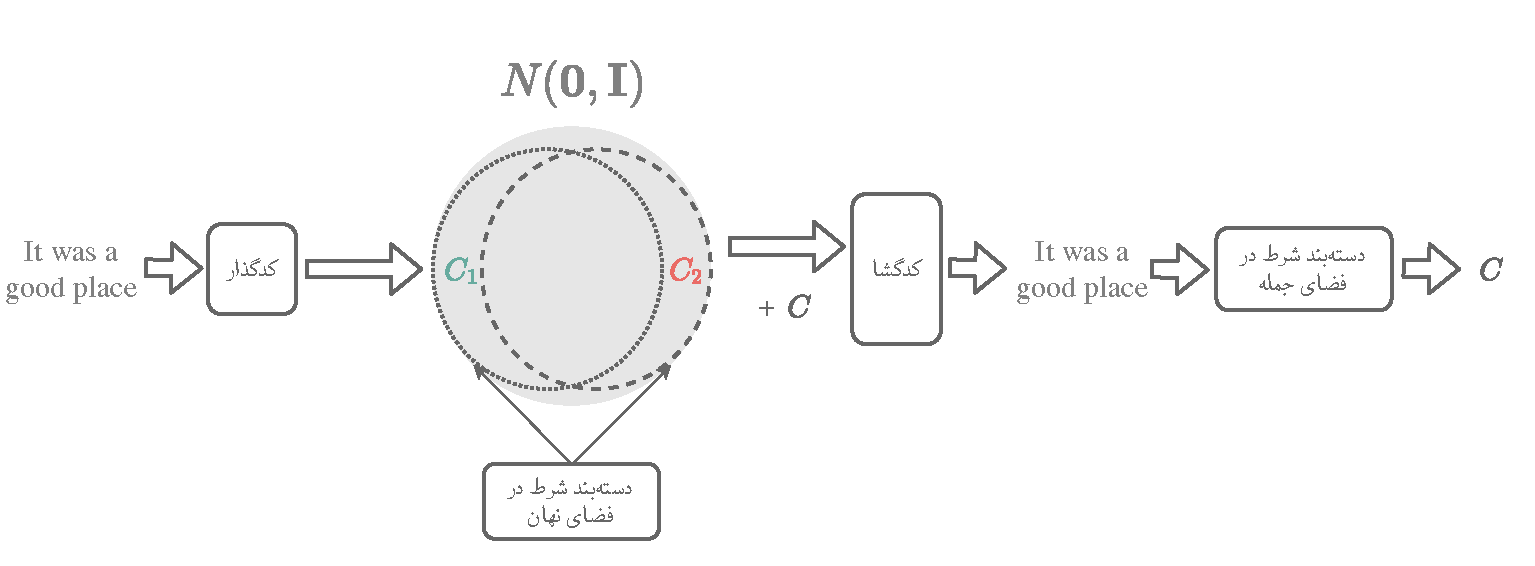
\includegraphics[width=1.\textwidth]{images/propdis.pdf}
        \caption{
            نمایی از مدل پیشنهادی دوم که فضای نهان از شرط مستقل است. همان طور که در شکل مشخص است، از یک \classifier{} برای تعیین برچسب شرط بردارهای فضای نهان بهره برده شده است. در مقابل، \encoder{} سعی در به اشتباه انداختن این \classifier{} خواهد داشت. در انتهای مدل نیز برای جلوگیری از عدم تطابق شرط با جمله تولیدی از یک \classifier{} جمله استفاده شده است.
        }
    \label{fig:chap4:prop2}
\end{figure}
\\
اگر \classifier{} را با $q_L(C|\bff{Z})$ نشان دهیم، توابع هزینه زیر اضافه خواهند شد:
\begin{gather}
    \mcal{L}(q_L) = -\expected_{(\bff{x},c) \sim p_\text{Data}, \bff{z} \sim q(\bff{Z}|\bff{x})} [\log q_L(c|\bff{z})]
    \\
    \mcal{L}(q) = -\lambda_\text{ENT} ~\expected_{\bff{x} \sim p_\text{Data}, \bff{z} \sim q(\bff{Z}|\bff{x})} [\mcal{H}_{q_L}(C)]
\end{gather}
که $q$ توزیع \encoder{} و  $\mcal{H}_{q_L}$ آنتروپی دسته‌بندی \classifier{} 
$q_L$ 
است. در واقع آنتروپی در زمانی بیشینه مقدار خود را دارد که \classifier{} به هیچ عنوان توانایی تشیخص برچسب را نداشته و با اطمینان ۵۰ درصد خروجی دهد.

برای جلوگیری از عدم تطابق جمله تولید شده با شرط، از یک دسته‌بند جمله نیز می‌توان بهره برد. به این صورت که از فضای نهان نمونه‌برداری کرده و سپس همراه با یک مقدار شرط تصادفی، توسط \decoder{} و همچنین به کارگیری روش \lr{Soft-argmax} (به منظور گذر گرادیان) که پیش‌تر توضیح داده شد،
 \decode{} 
 شده و تطابق جمله تولیدی با مقدار شرط مورد آزمون قرار می‌گیرد؛ به عبارت دیگر \decoder{} سعی در تولید جمله‌ای خواهد داشت که هزینه دسته‌بندی آن کم باشد.
 اگر \classifier{} جمله را با $q_D(C|\bff{X})$ نشان دهیم، توابع هزینه زیر اضافه خواهند شد:
 \begin{gather}
 \mcal{L}(q_D) = -\expected_{(\bff{x},c) \sim p_\text{Data}} [\log q_D(c|\bff{x})]
 \\
 \mcal{L}(G) = -\lambda_\text{CLS} ~\expected_{\bff{z} \sim p_\bff{Z}, c \sim p_C, \bff{x} \sim G(\bff{z};\tau)} [\log q_D(c|\bff{x})]
 \end{gather}
که $G(\bff{Z}; \tau)$ همان تابع \decoder{} است، با این تفاوت که به جای \greedydecoding{} از روش \lr{Soft-argmax} با پارامتر $\tau{}$ استفاده می‌شود.

در این فصل در ابتدا ضعف مدل‌های پیشین و در مواردی نیز با مثال تبیین شد. در ادامه معماری و روشی نوین ارائه شد تا بعضی از این نقاط ضعف را پوشش دهد. در فصل بعد ضمن معرفی معیارهای ارزیابی و دادگان مورد استفاده، مدل‌های پیشنهادی و مدل‌های پایه مورد ارزیابی و تحلیل قرار خواهند گرفت.

